\documentclass[aspectratio=169]{beamer}

% ProcRosetta: high-level presentation of the ICPM 2027 paper.

\usetheme{Madrid}
\usecolortheme{seahorse}
\usepackage{tikz}
\usetikzlibrary{positioning,fit,backgrounds,arrows.meta,calc,shapes.geometric}
\usepackage{booktabs}
\usepackage{pgfplots}
\pgfplotsset{compat=1.16}

\definecolor{procblue}{HTML}{2A78D6}
\definecolor{procgreen}{HTML}{1BAF7A}
\definecolor{procamber}{HTML}{D97E22}
\definecolor{procplum}{HTML}{8E5BC0}

\setbeamercolor{structure}{fg=procblue}
\setbeamercolor{frametitle}{bg=procblue!12, fg=procblue!50!black}
\setbeamertemplate{navigation symbols}{}
\setbeamertemplate{itemize items}[circle]

\newcommand{\keyc}[1]{\textbf{\textcolor{procblue}{#1}}}
\newcommand{\keyg}[1]{\textbf{\textcolor{procgreen!70!black}{#1}}}
\newcommand{\keya}[1]{\textbf{\textcolor{procamber!85!black}{#1}}}

\tikzset{
  iob/.style={draw=black!55, fill=black!4, rounded corners=2.5pt, align=center,
    inner sep=4pt, minimum height=9mm, font=\small},
  encb/.style={draw=procblue!75!black, fill=procblue!10, rounded corners=2.5pt,
    align=center, inner sep=4pt, minimum height=9mm, font=\small},
  decb/.style={draw=procgreen!70!black, fill=procgreen!12, rounded corners=2.5pt,
    align=center, inner sep=4pt, minimum height=9mm, font=\small},
  latb/.style={draw=procplum!75!black, fill=procplum!10, rounded corners=2.5pt,
    align=center, inner sep=4pt, minimum height=9mm, font=\small},
  flow/.style={-{Stealth[length=2.2mm]}, line width=0.9pt, draw=black!60},
  flab/.style={font=\scriptsize, text=black!60, align=center},
  stbg/.style={rounded corners=5pt, inner sep=2.5mm},
  stlab/.style={font=\scriptsize\itshape, inner sep=1.5pt},
}

\title[ProcRosetta]{\textbf{ProcRosetta}}
\subtitle{Aligning Event Logs, Process Trees, and Petri Nets\\in a Shared Latent Space with Grammar-Constrained Decoding}
\author[Berti, van der Aalst]{Alessandro Berti \and Wil M.P. van der Aalst}
\institute[PADS, RWTH]{Process and Data Science (PADS), RWTH Aachen University}
\date{ICPM 2027}

\begin{document}

% ---------------------------------------------------------------- 1
\begin{frame}
  \titlepage
\end{frame}

% ---------------------------------------------------------------- 2
\begin{frame}{The Problem}
  \begin{itemize}\setlength{\itemsep}{9pt}
    \item Process mining uses \keyc{three views} of the same behavior:
      \keyc{event logs}, \keyc{process trees}, \keyc{Petri nets}
    \item Every bridge between them is a \keya{dedicated algorithm}:
      discovery, conformance checking, model transformation
    \item Missing: a \keyg{common representation} in which the three views
      of one process are \keyg{the same point}
  \end{itemize}
  \vspace{4mm}
  \begin{center}
  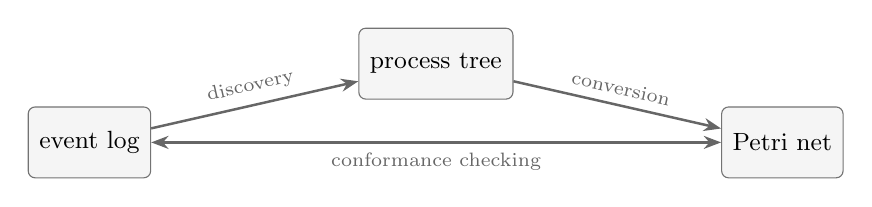
\begin{tikzpicture}[font=\small]
    \node[iob] (log) at (0,0) {event log};
    \node[iob] (tree) at (4.4,1.0) {process tree};
    \node[iob] (net) at (8.8,0) {Petri net};
    \draw[flow] (log) -- node[flab, above, sloped] {discovery} (tree);
    \draw[flow] (tree) -- node[flab, above, sloped] {conversion} (net);
    \draw[flow, {Stealth[length=2.2mm]}-{Stealth[length=2.2mm]}]
      (log) -- node[flab, below] {conformance checking} (net);
  \end{tikzpicture}
  \end{center}
\end{frame}

% ---------------------------------------------------------------- 3
\begin{frame}{The Goal}
  \begin{block}{One latent space of process behavior}
    Embed \keyc{logs}, \keyc{trees}, and \keyc{nets} so that three views of
    the \keyg{same process} land on \keyg{nearby points},
    and \keya{decode} any point back into a \keya{valid process model}.
  \end{block}
  \vspace{4mm}
  \begin{itemize}\setlength{\itemsep}{7pt}
    \item \keyc{RQ1}: do the three views of one process receive nearby embeddings?
    \item \keyc{RQ2}: can logs and nets be translated into \keyg{valid} process trees?
    \item \keyc{RQ3}: how does this compare with classical features and the Inductive Miner?
  \end{itemize}
  \vspace{3mm}
  \small The name: like the \keya{Rosetta stone}, the training data is the same
  content in three languages.
\end{frame}

% ---------------------------------------------------------------- 4
\begin{frame}{The Approach at a Glance}
  \begin{center}
  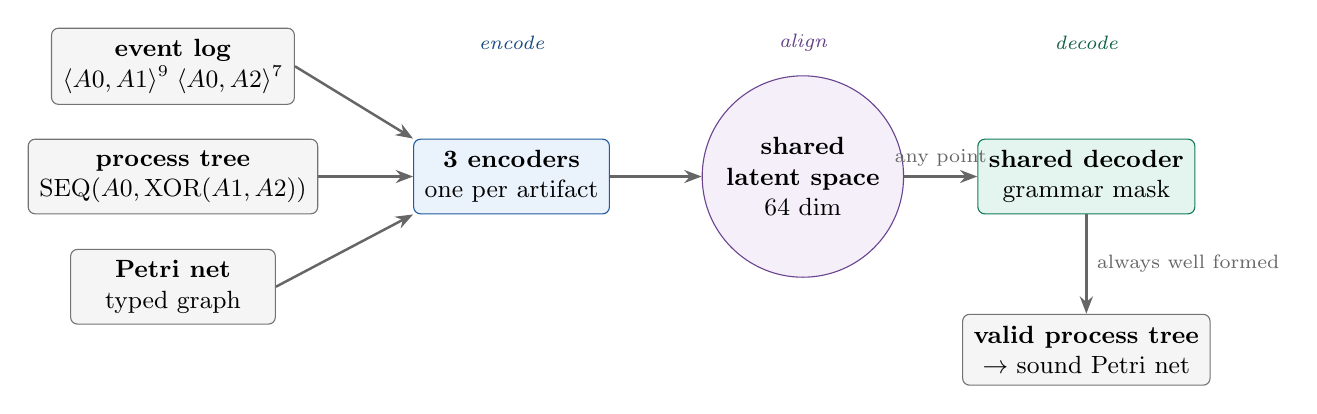
\begin{tikzpicture}[font=\small, node distance=3mm and 8mm]
    % inputs
    \node[iob, minimum width=26mm] (log) at (0,1.4) {\textbf{event log}\\$\langle A0,A1\rangle^{9}\;\langle A0,A2\rangle^{7}$};
    \node[iob, minimum width=26mm] (tree) at (0,0) {\textbf{process tree}\\$\mathrm{SEQ}(A0,\mathrm{XOR}(A1,A2))$};
    \node[iob, minimum width=26mm] (net) at (0,-1.4) {\textbf{Petri net}\\typed graph};
    % encoders
    \node[encb, minimum width=22mm] (enc) at (4.3,0) {\textbf{3 encoders}\\one per artifact};
    % latent space
    \node[latb, circle, minimum size=21mm] (lat) at (8.0,0) {\textbf{shared}\\\textbf{latent space}\\64 dim};
    % decoder
    \node[decb, minimum width=24mm] (dec) at (11.6,0) {\textbf{shared decoder}\\grammar mask};
    % output
    \node[iob, minimum width=23mm] (out) at (11.6,-2.2) {\textbf{valid process tree}\\$\to$ sound Petri net};
    \draw[flow] (log.east) -- (enc.north west);
    \draw[flow] (tree.east) -- (enc.west);
    \draw[flow] (net.east) -- (enc.south west);
    \draw[flow] (enc) -- (lat);
    \draw[flow] (lat) -- node[flab, above] {any point} (dec);
    \draw[flow] (dec) -- node[flab, right] {always well formed} (out);
    % stage labels
    \node[stlab, text=procblue!60!black] at (4.3,1.7) {encode};
    \node[stlab, text=procplum!70!black] at (8.0,1.7) {align};
    \node[stlab, text=procgreen!55!black] at (11.6,1.7) {decode};
  \end{tikzpicture}
  \end{center}
  \vspace{2mm}
  \begin{itemize}
    \item Same process $\Rightarrow$ views \keyc{pulled together};
      different processes \keya{pushed apart}
    \item Decoding realizes \keyg{discovery} (log $\to$ tree),
      \keyg{translation} (net $\to$ tree), \keyg{auto-encoding}
  \end{itemize}
\end{frame}

% ---------------------------------------------------------------- 5
\begin{frame}{Architecture}
  \begin{center}
  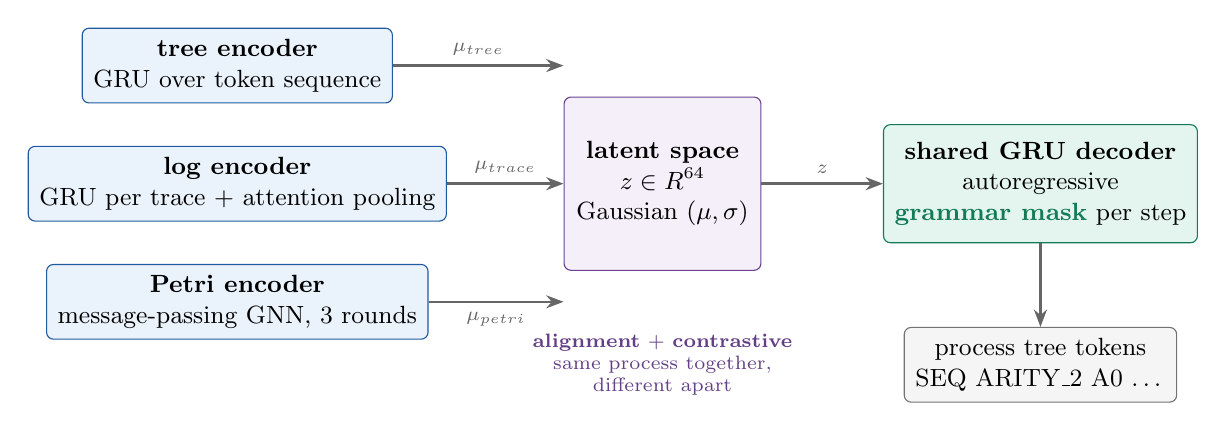
\begin{tikzpicture}[font=\small]
    % encoders
    \node[encb, minimum width=36mm] (te) at (0,1.5) {\textbf{tree encoder}\\GRU over token sequence};
    \node[encb, minimum width=36mm] (le) at (0,0) {\textbf{log encoder}\\GRU per trace $+$ attention pooling};
    \node[encb, minimum width=36mm] (pe) at (0,-1.5) {\textbf{Petri encoder}\\message-passing GNN, 3 rounds};
    % latent
    \node[latb, minimum width=25mm, minimum height=22mm] (lat) at (5.4,0)
      {\textbf{latent space}\\$z \in \mathbb{R}^{64}$\\Gaussian $(\mu, \sigma)$};
    % decoder
    \node[decb, minimum width=33mm, minimum height=15mm] (dec) at (10.2,0)
      {\textbf{shared GRU decoder}\\autoregressive\\\keyg{grammar mask} per step};
    \node[iob, minimum width=30mm] (out) at (10.2,-2.3) {process tree tokens\\SEQ ARITY\_2 A0 \ldots};
    \draw[flow] (te.east) -- node[flab, above, sloped] {$\mu_{tree}$} (lat.west |- te.east);
    \draw[flow] (le.east) -- node[flab, above] {$\mu_{trace}$} (lat.west);
    \draw[flow] (pe.east) -- node[flab, below, sloped] {$\mu_{petri}$} (lat.west |- pe.east);
    \draw[flow] (lat) -- node[flab, above] {$z$} (dec);
    \draw[flow] (dec) -- (out);
    % losses
    \node[font=\scriptsize, text=procplum!70!black, align=center] at (5.4,-2.3)
      {\textbf{alignment} $+$ \textbf{contrastive}\\same process together,\\different apart};
  \end{tikzpicture}
  \end{center}
  \vspace{1mm}
  \begin{itemize}
    \item Deliberately \keyc{small}: about \keyc{0.5M parameters}, trains in 30 min on CPU
  \end{itemize}
\end{frame}

% ---------------------------------------------------------------- 6
\begin{frame}{Grammar Masking: Validity by Construction}
  \begin{columns}[T]
  \begin{column}{0.52\textwidth}
    \begin{itemize}\setlength{\itemsep}{7pt}
      \item The decoder tracks \keyc{open node slots} and pending arities
      \item At every step, \keya{grammar-invalid tokens} get probability \keya{zero}
      \item Every terminated output \keyg{parses} into a process tree
      \item Deterministic conversion yields a \keyg{sound Petri net}
    \end{itemize}
  \end{column}
  \begin{column}{0.44\textwidth}
    \begin{center}
    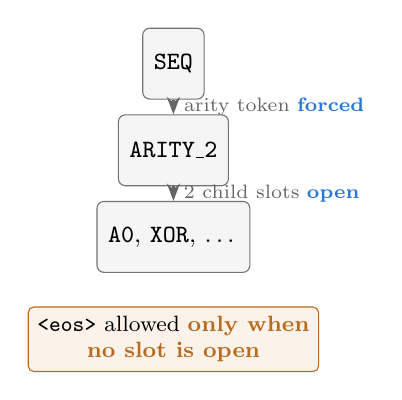
\begin{tikzpicture}[font=\footnotesize]
      \node[iob] (s1) at (0,2.2) {\texttt{SEQ}};
      \node[iob] (s2) at (0,1.1) {\texttt{ARITY\_2}};
      \node[iob] (s3) at (0,0) {\texttt{A0}, \texttt{XOR}, \ldots};
      \draw[flow] (s1) -- node[flab, right] {arity token \keyc{forced}} (s2);
      \draw[flow] (s2) -- node[flab, right] {2 child slots \keyc{open}} (s3);
      \node[draw=procamber!85!black, fill=procamber!10, rounded corners=2pt,
        font=\footnotesize, align=center] at (0,-1.3)
        {\texttt{<eos>} allowed \keya{only when}\\\keya{no slot is open}};
    \end{tikzpicture}
    \end{center}
  \end{column}
  \end{columns}
  \vspace{3mm}
  \begin{block}{}
    \centering \keyg{100\%} of 2{,}048 test decodes: valid tree, convertible to a Petri net
  \end{block}
\end{frame}

% ---------------------------------------------------------------- 7
\begin{frame}{Training and Validation Data}
  \begin{columns}[T]
  \begin{column}{0.55\textwidth}
    \textbf{Synthetic paired triples} (correspondence by construction):
    \vspace{2mm}
    \begin{enumerate}\setlength{\itemsep}{5pt}
      \item \keyc{sample} a random process tree\\(SEQ, XOR, AND; depth $\le 3$; $\le 30$ activities)
      \item \keyc{simulate} it into an event log\\(16 traces per sample)
      \item \keyc{convert} it into a Petri net\\(deterministic, via PM4Py)
    \end{enumerate}
  \end{column}
  \begin{column}{0.41\textwidth}
    \begin{center}
    \begin{tabular}{lr}
      \toprule
      Split & Triples \\
      \midrule
      \keyc{Training} & 4{,}000 \\
      \keyc{Validation} & 512 \\
      \keyc{Test} & 512 \\
      \bottomrule
    \end{tabular}
    \end{center}
    \vspace{2mm}
    \small Fixed seed, disjoint splits.\\
    Avg.\ tree size $\approx 10$ nodes.
  \end{column}
  \end{columns}
\end{frame}

% ---------------------------------------------------------------- 8
\begin{frame}{Training Loss}
  All three artifacts of a triple decode to the \keyc{same target tree}:
  \begin{equation*}
    \mathcal{L} \;=\; \underbrace{\mathcal{L}_{\mathit{tree}\to\mathit{tree}}
      + \mathcal{L}_{\mathit{log}\to\mathit{tree}}
      + \mathcal{L}_{\mathit{petri}\to\mathit{tree}}}_{
      \textcolor{procblue}{\textbf{reconstruction and translation}}}
    \;+\; 0.1\,\underbrace{\mathcal{L}_{\mathit{align}}}_{
      \textcolor{procplum!80!black}{\textbf{pull together}}}
    \;+\; 0.1\,\underbrace{\mathcal{L}_{\mathit{contrastive}}}_{
      \textcolor{procamber!85!black}{\textbf{push apart}}}
    \;+\; 0.001\,\mathcal{L}_{\mathit{KL}}
  \end{equation*}
  \vspace{1mm}
  \begin{itemize}\setlength{\itemsep}{6pt}
    \item \keyc{Decode losses}: grammar-masked cross-entropy (teacher forcing)
      for reconstruction (tree $\to$ tree) and the two translations
      (log $\to$ tree, Petri net $\to$ tree)
    \item \keyc{Alignment}: squared distance between the latent means of the
      three views: \keyg{same process, same point}
    \item \keya{Contrastive} (CLIP style): each artifact must be most similar to
      its \keyg{own counterpart} in the batch: \keya{different processes apart}
    \item \keyc{KL}: weak pull toward a standard normal keeps the space
      \keyg{bounded and smooth}
  \end{itemize}
\end{frame}

% ---------------------------------------------------------------- 9
\begin{frame}{Evaluation: How}
  All on the \keyc{held-out test split} (512 triples), best-validation checkpoint:
  \vspace{3mm}
  \begin{itemize}\setlength{\itemsep}{8pt}
    \item \keyc{Decode quality}: validity, exact match, edit distance,
      \keyg{behavioral distance} of decoded model vs.\ source log
    \item \keyc{Discovery quality}: log $\to$ model vs.\ the \keya{Inductive Miner},
      scored by alignment-based fitness and precision
    \item \keyc{Embedding quality}: does latent distance correlate with
      \keyg{behavioral distance}? vs.\ 7 baselines incl.\ PetriNet2Vec
    \item \keyc{Cross-modal retrieval}: given a net, find its log among 512 candidates
  \end{itemize}
\end{frame}

% ---------------------------------------------------------------- 9
\begin{frame}{Evaluation: Results}
  \begin{columns}[T]
  \begin{column}{0.5\textwidth}
    \begin{itemize}\setlength{\itemsep}{6pt}
      \item \keyg{100\%} valid, Petri-convertible decodes from all modalities
      \item Discovery: F1 \keyc{0.787} vs.\ \keya{0.857} Inductive Miner\\
        {\small (92\% of IM, on IM's home turf)}
      \item Embedding quality via $\rho$ $=$ \keyc{Spearman rank correlation}:
        do \keyg{behaviorally close} logs get \keyg{close embeddings}?
      \item Retrieval top-1: \keyc{14 to 44\%} vs.\ \keya{0.2\%} chance
    \end{itemize}
    \vspace{2mm}
    \small Decoded models: behaviorally \keyg{twice as close} to their source
    as unrelated ones; the three encoders converge to \keyc{one geometry}.
  \end{column}
  \begin{column}{0.46\textwidth}
    \begin{center}
    \small
    \begin{tabular}{lcc}
      \toprule
      Decode from & Valid & Exact \\
      \midrule
      tree  & \keyg{100\%} & 48\% \\
      log   & \keyg{100\%} & 40\% \\
      net   & \keyg{100\%} & 36\% \\
      \bottomrule
    \end{tabular}
    \vspace{3mm}

    \small
    \begin{tabular}{lrc}
      \toprule
      Log representation & Dim. & $\rho$ \\
      \midrule
      \keyc{ProcRosetta} (learned) & \keyc{64} & 0.630 \\
      directly-follows relations & 332 & 0.736 \\
      trace-variant distribution & 2{,}548 & 0.614 \\
      \bottomrule
    \end{tabular}
    \end{center}
    \vspace{1mm}
    \small A compact \keyc{64-dim} learned vector rivals feature vectors
    \keya{5 to 40$\times$ larger} that partly \keya{define} the target distance.
  \end{column}
  \end{columns}
\end{frame}

% ---------------------------------------------------------------- 10
\begin{frame}{What Can Be Improved: Data}
  \begin{itemize}\setlength{\itemsep}{10pt}
    \item \keya{Only synthetic} data: all triples come from small random
      block-structured trees, so results hold \keyc{in distribution} only;
      training and validating on \keyc{real-life logs} and model collections
      would test whether the space transfers to realistic behavior
    \item \keya{Clean logs}: every log is a perfect, noise-free playout of its
      tree; real logs contain \keyc{noise, incomplete cases, deviations,
      long-tail variants}, and a model trained on them would have to
      \keyc{abstract} instead of just compress
    \item \keya{Possible near-duplicates} across splits: splits are random, so
      a test behavior can resemble a training behavior and
      \keyc{inflate exact-match rates}; explicit \keyc{behavioral deduplication}
      would make the numbers stricter
    \item \keya{Single seed}: one data configuration, one trained model;
      \keyc{multi-seed runs} would quantify how stable the results are
  \end{itemize}
\end{frame}

% ---------------------------------------------------------------- 11
\begin{frame}{What Can Be Improved: Architecture}
  \begin{itemize}\setlength{\itemsep}{12pt}
    \item \keya{Small GRU-based encoders and decoder} (about 0.5M parameters):
      \keyc{scaling} them, or replacing GRUs with \keyc{transformers},
      should close part of the gap to the Inductive Miner,
      especially on longer trees and larger logs
    \item \keya{Block-structured output only}: the decoder can express only what
      a process tree can express; a richer \keyg{sound} target language such as
      \keyc{POWL} (partially ordered workflow models) needs just a new
      \keyc{prefix grammar} and deterministic Petri-net conversion,
      the rest of the framework stays unchanged
    \item \keya{Only three modalities}: the latent space is open;
      attaching \keyc{new encoders}, e.g.\ for \keyg{natural-language}
      process descriptions or BPMN, would let text, logs, and models
      meet in \keyc{one space}, closer to a true Rosetta stone
  \end{itemize}
\end{frame}

% ---------------------------------------------------------------- 12
\begin{frame}{Takeaway}
  \begin{block}{}
    \centering
    \keyc{One latent space}, three artifact types,
    \keyg{valid models by construction}.
  \end{block}
  \vspace{4mm}
  \begin{itemize}\setlength{\itemsep}{8pt}
    \item Three encoders converge to \keyc{one geometry} of process behavior (RQ1)
    \item Grammar masking: \keyg{100\%} valid, sound outputs (RQ2)
    \item Learned translation reaches \keyc{92\%} of the Inductive Miner F1;
      64-dim embeddings rival much larger deterministic features (RQ3)
  \end{itemize}
  \vspace{4mm}
  \centering\small Code, data generator, and evaluation suite:\\
  \url{https://github.com/fit-alessandro-berti/proc-rosetta}
\end{frame}

% ================================================================ appendix
\appendix

\begin{frame}
  \centering
  {\LARGE \textbf{\textcolor{procblue}{Appendix}}}\\[3mm]
  {\large Detailed Evaluation Results}\\[5mm]
  \small All numbers on the held-out test split (512 triples).
\end{frame}

% ---------------------------------------------------------------- A2
\begin{frame}{Appendix: Decode Quality}
  Greedy decoding from each latent source (512 samples each):
  \vspace{2mm}
  \begin{center}
  \small
  \begin{tabular}{lcccc}
    \toprule
    Latent source & Valid tree & Exact tree & Norm.\ edit $\downarrow$ & Behavior $L_1$ $\downarrow$ \\
    \midrule
    $\mu_{\mathit{tree}}$ (tree encoder)   & \keyg{100\%} & \keyc{48.4\%} & \keyc{0.178} & \keyc{0.675} \\
    $\mu_{\mathit{trace}}$ (log encoder)   & \keyg{100\%} & 40.0\% & 0.287 & 0.755 \\
    $\mu_{\mathit{petri}}$ (Petri encoder) & \keyg{100\%} & 35.9\% & 0.282 & 0.839 \\
    $\mu_{\mathit{fused}}$ (mean of three) & \keyg{100\%} & 44.3\% & 0.230 & 0.713 \\
    \bottomrule
  \end{tabular}
  \end{center}
  \vspace{3mm}
  \begin{itemize}\setlength{\itemsep}{5pt}
    \item \keyc{Behavior $L_1$}: distance between the original log and traces
      simulated from the decoded model, range $[0,2]$;
      two \keya{unrelated} test logs average \keya{1.566}
    \item Ordering is intuitive: the tree embedding keeps the most information,
      then the log, then the \keya{label-free} Petri net structure
  \end{itemize}
\end{frame}

% ---------------------------------------------------------------- A3
\begin{frame}{Appendix: Discovery Quality vs.\ Inductive Miner}
  \begin{columns}[T]
  \begin{column}{0.5\textwidth}
    \vspace{4mm}
    \begin{itemize}\setlength{\itemsep}{7pt}
      \item Each of the 512 test logs: encode, decode a tree, convert to a
        Petri net; scored by \keyc{alignment-based} fitness and precision
      \item Test logs are noise-free playouts of block-structured trees:
        the Inductive Miner's \keya{best case} (rediscovery guarantee,
        fitness 1.0)
      \item ProcRosetta compresses the whole log into \keyc{one 64-dim vector},
        no search or replay, and still reaches \keyc{92\%} of the IM's F1
    \end{itemize}
  \end{column}
  \begin{column}{0.46\textwidth}
    \begin{center}
    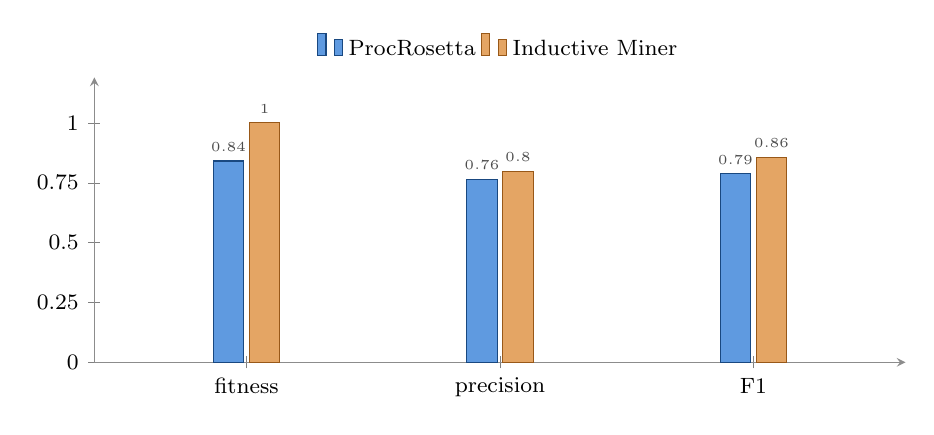
\begin{tikzpicture}
    \begin{axis}[
      ybar, bar width=11pt,
      width=0.98\linewidth, height=5.2cm,
      ymin=0, ymax=1.19,
      symbolic x coords={fitness, precision, F1},
      xtick=data,
      ytick={0,0.25,0.5,0.75,1.0},
      axis lines=left, axis line style={black!45},
      enlarge x limits=0.3,
      ticklabel style={font=\footnotesize},
      legend style={draw=none, fill=none, font=\footnotesize, at={(0.5,1.02)},
        anchor=south, legend columns=2},
      nodes near coords,
      every node near coord/.append style={font=\tiny, color=black!70},
    ]
    \addplot[fill=procblue!75, draw=procblue!60!black]
      coordinates {(fitness,0.841)(precision,0.763)(F1,0.787)};
    \addlegendentry{ProcRosetta}
    \addplot[fill=procamber!70, draw=procamber!70!black]
      coordinates {(fitness,1.000)(precision,0.797)(F1,0.857)};
    \addlegendentry{Inductive Miner}
    \end{axis}
    \end{tikzpicture}
    \end{center}
  \end{column}
  \end{columns}
\end{frame}

% ---------------------------------------------------------------- A4
\begin{frame}{Appendix: Embedding Quality}
  Spearman $\rho$ vs.\ behavioral distance over all 130{,}816 log pairs;
  NN $=$ mean behavioral distance to the nearest embedding neighbor
  (random pair: 1.566):
  \vspace{2mm}
  \begin{center}
  \footnotesize
  \begin{tabular}{llrrr}
    \toprule
    Method & Type & Dim. & $\rho$ $\uparrow$ & NN $\downarrow$ \\
    \midrule
    Directly-follows distribution$^\dagger$ & log features & 332 & \keya{0.736} & 0.784 \\
    PetriNet2Vec & learned (net) & 64 & 0.643 & 1.115 \\
    Activity counts & log features & 20 & 0.635 & 0.946 \\
    \keyc{ProcRosetta} $\mu_{\mathit{trace}}$ & learned (log) & \keyc{64} & 0.630 & \keyc{0.794} \\
    \keyc{ProcRosetta} $\mu_{\mathit{fused}}$ & learned (all) & \keyc{64} & 0.628 & 0.804 \\
    Trace-variant distribution$^\dagger$ & log features & 2{,}548 & 0.614 & \keya{0.781} \\
    \keyc{ProcRosetta} $\mu_{\mathit{tree}}$ & learned (tree) & \keyc{64} & 0.611 & 0.836 \\
    \keyc{ProcRosetta} $\mu_{\mathit{petri}}$ & learned (net) & \keyc{64} & 0.574 & 0.913 \\
    Eventually-follows distribution & log features & 347 & 0.412 & 0.881 \\
    \bottomrule
  \end{tabular}
  \end{center}
  \vspace{2mm}
  \small $^\dagger$ shares components with the behavioral-distance definition:
  a \keya{skyline}, not a fair competitor. Among the rest, ProcRosetta's log
  embedding is the \keyc{strongest all-round performer} at only 64 dimensions.
\end{frame}

% ---------------------------------------------------------------- A5
\begin{frame}[fragile]{Appendix: Cross-Modal Retrieval}
  \begin{columns}[T]
  \begin{column}{0.46\textwidth}
    \vspace{2mm}
    \begin{center}
    \small
    \begin{tabular}{lccc}
      \toprule
      Query $\to$ target & Top-1 & MRR & Rank \\
      \midrule
      tree $\to$ Petri net & \keyc{44.3\%} & 0.523 & 36.2 \\
      Petri net $\to$ tree & 34.2\% & 0.442 & 38.0 \\
      tree $\to$ log & 29.3\% & 0.383 & 32.4 \\
      log $\to$ tree & 25.6\% & 0.354 & 33.2 \\
      Petri net $\to$ log  & 15.4\% & 0.236 & 49.4 \\
      log $\to$ Petri net  & 14.1\% & 0.236 & 48.2 \\
      \bottomrule
    \end{tabular}
    \end{center}
    \vspace{2mm}
    \small
    \keyc{MRR} $=$ mean reciprocal rank: the average of $1 / \mathrm{rank}$
    of the true counterpart; \keyc{1.0} means it is always ranked
    \keyg{first}, \keyc{0.5} means it is typically \keyg{second}.\\[2mm]
    Chance level: top-1 $=$ \keya{0.2\%}, mean rank $\approx$ \keya{256}.
  \end{column}
  \begin{column}{0.5\textwidth}
    \begin{center}
    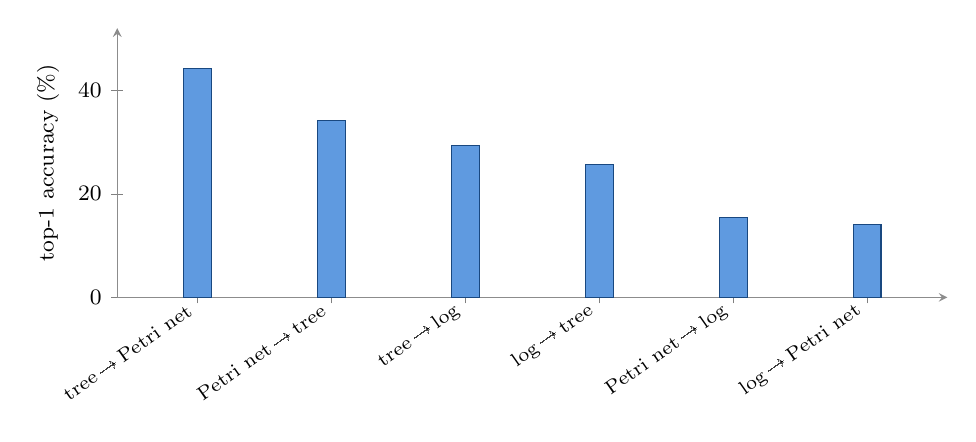
\begin{tikzpicture}
    \begin{axis}[
      ybar, bar width=10pt,
      width=\linewidth, height=5.0cm,
      ymin=0, ymax=52, ylabel={top-1 accuracy (\%)},
      xtick={1,2,3,4,5,6},
      xticklabels={{tree\,\textrightarrow\,Petri net},{Petri net\,\textrightarrow\,tree},
        {tree\,\textrightarrow\,log},{log\,\textrightarrow\,tree},
        {Petri net\,\textrightarrow\,log},{log\,\textrightarrow\,Petri net}},
      x tick label style={rotate=35, anchor=east, font=\scriptsize},
      ylabel style={font=\footnotesize},
      axis lines=left, axis line style={black!45},
      enlarge x limits=0.12,
      ticklabel style={font=\footnotesize},
    ]
    \addplot[fill=procblue!75, draw=procblue!60!black]
      coordinates {(1,44.3)(2,34.2)(3,29.3)(4,25.6)(5,15.4)(6,14.1)};
    \end{axis}
    \end{tikzpicture}
    \end{center}
    \small Instance-level matching: the correct counterpart among
    \keyc{512 candidates}, \keyg{70 to 220$\times$} above chance.
  \end{column}
  \end{columns}
\end{frame}

\end{document}
